%
%
\documentclass{article}
\usepackage{amsmath}
\usepackage{graphicx}
\usepackage{color}
\usepackage{caption}
\usepackage{amsfonts}
%\usepackage[margin=3cm]{geometry}
\usepackage{tikz}
\newcommand{\cE}{\mathcal{E}}                               %

\begin{document}

\title{Initial summary of project and progress so far}
\author{Dominic Skinner}
\maketitle
\section*{Introduction}
Consider a semi-infinite crack in a solid with an incompressible fluid 
being driven into the crack. The solid above the crack is like a beam
and we treat the solid as an elastic solid.

What we are interested in is the asymptotics as we approach the tip
of the crack. This means that there are two asymptotic regimes that 
we are interested in. The first is the lubrication limit from fluid
dynamics. The second is the elastic fracure region from solid mechanics.

\section{Set up}
\begin{figure}[!ht]\centering
\caption{Set up of problem}
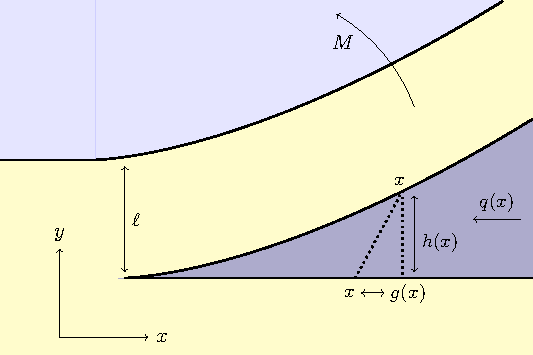
\includegraphics{Fig1.pdf}
\end{figure}
We look for a steadily propagating solution 
\[h \equiv h(x-ct)\]
In the fluid we use standard lubrication results to find that 
\[ q = - \frac{1}{12\mu}\frac{dp}{dx} h^3\] 
Use conservation of mass, i.e.
$\displaystyle \frac{\partial q}{\partial x} + 
\frac{\partial h}{\partial t} =0$ to get
\begin{equation}
p' = \frac{\lambda}{h^2}
\end{equation}
Where $\lambda$ is a constant which essentially measures the speed
of propagation.
This governs the fluid. In the solid, we use results from elasticity.
Let $P=\sigma_y$ be the stress and let $\tau_{xy} =0$ i.e. no shear\footnote{
It can be shown that the shear is an order of magnitude smaller than the pressure}.
Then
\[ \left( \begin{array}{c} P \\ M \end{array} \right) =
 \left( \begin{array}{c} P \\ 0 \end{array} \right) =
 \left( \begin{array}{c} \sigma_y \\ \tau_{xy} \end{array} \right) =
C \int_0^{\infty} \left(
\begin{array}{cc} K_{11}(z-x) & K_{12}(z-x) \\ K_{21}(z-x) & K_{22}(z-x) \end{array}
\right)
 \left( \begin{array}{c} g'(z) \\ h'(z) \end{array} \right) dz
\]
Where $C$ is a (known) constant, and the $K_{ij}$ have (ugly) analytic expressions.
\subsubsection*{Boundary Conditions}

\begin{figure}[!ht]\centering
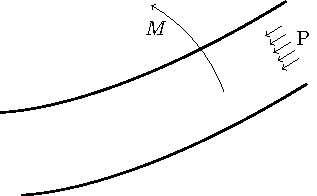
\includegraphics{Fig2.pdf}
\end{figure}
At $\infty$ have from fracture mechanics
\[ g' \to \frac{1}{4}(-P+6M)\]
\[ h'' \to 3M\]
But at 0 this depends on the fracture mechanics.

In the no fracture case (Think of two separate solids sitting on top of each
other), the solution obeys lubrication right to 0. I.e. 
\begin{alignat*}{2}
h &\sim x^{2/3}  \qquad & p'\sim x^{-4/3} \\
h' & \sim x^{-1/3} \qquad &  p\sim x^{-1/3}
\end{alignat*}
In the fracture case: ``Axioms'' of fracture mechanics imply that
\[h \approx Kx^{1/2} \]
Where $K$ is the toughness.
Possible ``Dependent Variables''
\begin{itemize}
\item at $\infty$ have $P$, $M$. Where $P$ is the only
	one we really care about, as we can set $M=0$. After rescaling 
	$x,h$ it is possible to assume $P=1$.
\item At 0, have speed\footnote{Well, a parameter which essentially is a 
	scaled measure of the speed} $\lambda$ and toughness $K$.
\end{itemize}
Given a fixed toughness $K$, propagation occurs at $\lambda(K)$ 
(and vica-versa).

What we really want is to find $\lambda$ for $K=0$, and then the 
``small toughness'' solution for $K\approx0$.
\begin{figure}[!ht]\centering
\caption{Why we are interested in this problem}
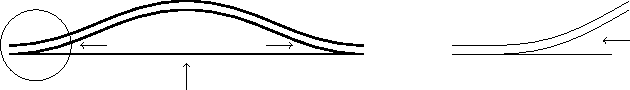
\includegraphics{Fig3.pdf}
\end{figure}

\section{Zero toughness solution}
Recall we have
\[ \left( \begin{array}{c} \sigma_y \\ \tau_{xy} \end{array} \right) =
C \int_0^{\infty} \left(
\begin{array}{cc} K_{11} & K_{12} \\ K_{21} & K_{22} \end{array}
\right)
 \left( \begin{array}{c} g' \\ h' \end{array} \right) dz
\]
In the complicated geometry. Looking close to the crack tip can move into a 
much simpler geometry where the solid extends infinitely in the $y$ direction.
\begin{figure}[!ht]\centering
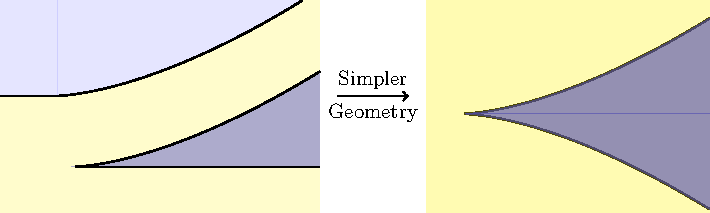
\includegraphics{Fig5.pdf}
\end{figure}
$K(\lambda_0)=0$.
In this simpler geometry, $\sigma = p$ and this depends only on $h'$,
since we can ignore non singular terms near the crack tip.
\[ \implies p(x) = \int_0^{\infty} \frac{h'(z)}{z-x}dz \]
i.e. $p$ is the Hilbert transform of $h'$. Also have 
\[p' = \frac{\lambda}{h^2} \]
so try $h=x^{\alpha}\implies$
\begin{align*}
p  &\sim x^{\alpha-1}\\
p' &\sim x^{-2\alpha}
\end{align*}
\[\implies -2\alpha = \alpha -2 \]
or $\alpha = 2/3$ as claimed earlier,
where we have made use of the Hilbert transform
\[ \int_0^{\infty} \frac{z^{s-1}}{z-x} dz = -\pi \cot(\pi s) z^{s-1}\]
So starting with a solution $h_0 = A_0x^{2/3}+ \dots$ near the
crack tip, have that 
\[ p_0(x) = \int_0^{\infty} \frac{48(z-x)^2-64}{(z-x)((z-x)^2+4)^3}
\; \frac{2A_0}{3} z^{-1/3} dz = \dots \approx \frac{2A_0}{3}\int_0^{\infty} 
\frac{z^{-1/3}}{z-x}dz\]
and therefore get that
\[p_0 = -\frac{3\lambda_0}{A_0^2x^{1/3}} + \dots\] 

\section{Perturbing the Zero toughness solution}
Suppose that we have a solution for $\lambda_0$, $K(\lambda_0)=0$
(and $h_0,g_0,p_0$). We want to now consider when $K\approx0$, 
$\lambda \approx \lambda_0$ i.e. perturb this solution.

$K=0$ solution:
\begin{align*}
h_0 &= A_0x^{2/3}+ \dots \\
p'_0 &= \frac{\lambda_0}{A_0^2x^{4/3}}+ \dots \\
p_0 &= -\frac{3\lambda_0}{A_0^2x^{1/3}}+ \dots 
\end{align*}
Which are the leading order terms as $x\to0$.
Now, given $(g_0,h_0)$ perturb:
\begin{align*}
g &= g_0 + \mathcal{E}(K) \; g_1 + \dots \\
h &= h_0 + \mathcal{E}(K) \; h_1 + \dots \\
p &= p_0 + \mathcal{E}(K) \; p_1 + \dots \\
\lambda &= \lambda_0 + \mathcal{E}(K) \; \lambda_1 + \dots 
\end{align*}
Where we assume $\mathcal{E}(K)$ is small, for example 
$\mathcal{E}(K) = K$, but we need not have this in general.
In this perturbation, we get two regions close to the fracture, 
the lubrication region and the fracture region. 
\begin{figure}[!ht]\centering
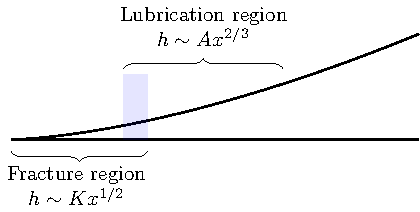
\includegraphics{Fig6.pdf}
\end{figure}

\subsubsection*{Lubrication region}
\[h(x) = A(K)x^{2/3} + \dots\]
\[A(K) = \left(\frac{243\lambda(K)^2}{4\pi^2}\right)^{1/6}
=\underbrace{A_0}_{\mbox{in } h_0} + 
\underbrace{\frac{A_0\lambda_1}{3\lambda_0}\cE(K)}_{\mbox{in } 
h_1 \mbox{ term}} + \dots\]
and so
\[ h = \underbrace{A_0 x^{2/3}}_{h_0} + 
\underbrace{\left( \frac{A_0\lambda_1}{3\lambda_0} x^{2/3} +x^s\right)  }_{h_1} 
\cE(K) + \dots \]
Solve for $h_1$ via $p' = \lambda/h^2$
\[ (p_0 + \cE p_1)' = \frac{\lambda_0 + \cE\lambda_1}{(h_0+\cE h_1)^2} \]
At order $\cE$
\[\lambda_1 = h_0^2 p_1' + 2h_0h_1p_0'\]
So
\[p_1' = \frac{\lambda_1}{3A_0^2}x^{-4/3} - \frac{4\pi}{9\sqrt{3}}x^{s-2}\]
Then do the Hilbert transform
\[ p_1 =
 \int_0^{\infty} \left(
\begin{array}{cc} K_{11} & K_{12} \end{array}
\right)
 \left( \begin{array}{c} g_1' \\ h_1' \end{array} \right) dz
\]
Plugging into the earlier expression, find that $s\approx 0.138773$.
So in the lubrication region, $h$ scales like $Ax^{2/3}+Bx^{0.13867\dots}$

\subsubsection*{Fracture region}
Here pretend no free surface as we are zoomed in far enough that we see
the solid in every direction.
$h\sim Kx^{1/2}$ at $x\to0$. We can remove $\lambda, K$ by making the problem
dimensionless.
\[ p \to \Pi \qquad h \to \eta \qquad x \to \xi \]
($\lambda = K = 1$)
\[ \eta(\xi) = \tilde{A}\xi^{2/3} + C \xi^{t}\]
$t$ some constant. But doing the same thing as earlier, compare results
of $\Pi'=\frac{1}{\eta^2}$ and $\Pi=$ Hilbert transform of $\eta'$.
\begin{figure}[!ht]\centering
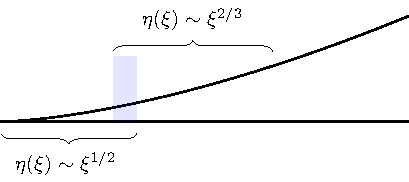
\includegraphics{Fig7.pdf}
\end{figure}

From this, we find that $t=s=0.1386\dots$. Redimensionalising, get that
\[ h(x) = \mathcal{O} x^{2/3} + K^{4-6s}x^s\]
i.e. $\cE(K)=K^{4-6s}$. This tells us that 
\[\lambda = \lambda_0 + K^{4-6s}\lambda_1 \]
But we don't know $\lambda_1$.
Well, get it out of linearized problem:
\[ \left\{ \begin{array}{ccc}
\lambda_1 &=& h_0^2p_1'+2h_0p_0'h_1 \\[6pt]
\left(\begin{array}{c} p_1 \\ 0 \end{array} \right)
& =&  \int \left(
\begin{array}{cc} K_{11} & K_{12} \\ K_{21} & K_{22} \end{array}
\right)
 \left( \begin{array}{c} g_1' \\ h_1' \end{array} \right)
 
\end{array}
\right.
\]
What are the boundary conditions?
\[h_1'' \to 0, \qquad g_1' \to 0 \qquad \mbox{at } x \to \infty \;\;(??)\]
\[ \cE(K)h_1 \to Kx^{1/2} \mbox{  at } x\to 0 \]

\section{Numerical Methods}
Given $\lambda$ you can find $K(\lambda)$ via running a numerical simulation.
Then it is essentially Newtons method to find $\lambda_0$ s.t. 
\begin{figure}[!ht]\centering
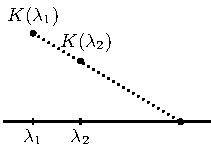
\includegraphics{Fig4.pdf}
\end{figure}
$K(\lambda_0)=0$.

What is observed is $\lambda - \lambda_0 \approx K^3$ (or is it $K^{3.14\dots}$
very difficult to tell numerically).

Discretize: First try to represent $h_1', g_1'$ as piecewise linear functions.
Recall that $K_{ij}(z-x)\,(az+b)$ has an analytic expression.
This can cause issues near the tip where $h' \sim x^{-1/2}$. So for half the
panels (near tip) use scheme $g', h' \sim ax^{1/2} + bx^{-1/2}$ and for the
rest of the panels use $g',h' \sim ax +b$.
\begin{figure}[!ht]\centering
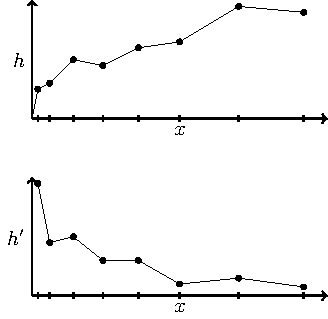
\includegraphics{Fig8.pdf}
\end{figure}
%
%
% References/Bibliography //////////////////////////////////////////////\\/////////////
%
%\clearpage 
%\begin{thebibliography}{9}  
%
%\bibitem{Pedlosky}
%Pedlosky, J.,
%\emph{Geophysical Fluid Dynamics,}
%Springer-Verlag,
%1979.
%
%
%\end{thebibliography}
\end{document}

